\chapter{Introduction}\label{ch:1}

%section 1.1 begins %%%%%%%%%%%%%%%%%%%%%%%%%%%%%%%%%%%%%%%%%%%%%%%%%%%%%%%%%%%%%%%%%%%%
\section{An interest sparked} \label{1.1}
The summer of 2004 marked the first time I, as a then undergraduate student, had ever set foot on Surinamese soil. The purpose of the trip was to collect language data on the \ili{English}-\isi{lexicon} creoles spoken in the country. In analysing the data collected, I began to unearth various correspondences between the phonetic shapes of words of \ili{English} origin and their reflexes across \ili{Saramaccan}, \ili{Sranan}, and \ili{Aukan}, hereafter \textsc{ssa}.

In March of 2007, I, as a graduate student supervising an undergraduate fieldtrip, went to \isi{Suriname} again. On that occasion, I was fortunate enough to be able to collect additional data from other \textsc{ssa}  settlements not previously visited during the 2004 fieldtrip. On this occasion, the goal was to determine to what degree the phenomena noticed on the 2004 fieldtrip were similar across different groups of \textsc{ssa}  speakers. I noticed the same phonetic correspondences as well as new ones across the various \textsc{ssa}  reflexes and their \ili{English} cognates.

One correspondence observed was the production and non-production of /r/ in post-vocalic positions. Some \textsc{ssa}  words such as \ili{Sranan}'s \emph{more} [moro], \ili{Saramaccan}'s \emph{work} [woroko] and \ili{Aukan}'s  \emph{gutter} [gotro] suggested that the \ili{English} input forms had a postvocalic /r/, hereafter \textsc{pvr}. However, other words such as \ili{Sranan}'s \emph{four} [fɔ], \ili{Saramaccan}'s \emph{finger} [fɪŋga] and \ili{Aukan}'s \emph{horse} [asɪ] suggested that other \ili{English} input forms lacked a post-vocalic /r/; I was fascinated and my fascination led me to ask three questions:

\begin{enumerate}
\item Was \textsc{ssa}  influenced by both /r/-full and /r/-less \ili{British} Isles \ili{English} \isi{dialects}?
\item Was \textsc{ssa}  influenced by both /r/-full and /r/-less \ili{British} Isles \ili{English} \isi{dialects}?
\item Was the combination /r/-fullness and /r/-lessness a purely \ili{Sranan} phenomenon?
\end{enumerate}

I had a desire to know more; I needed to know the exact origin of the patterns of correspondence and lack of correspondence thereof, with rhotic \isi{dialects} of \ili{English} and \textsc{ssa}. I also needed to ascertain why these and other patterns presented themselves across all three creoles. This linguistic curiosity led to my perusing both historical and historical-linguistic works about \textsc{ssa}  and \isi{Suriname}; some of these included: \citet{Bridenbaugh68},  \citet{Esposito82},   \citet{Hoefte98}, \citet{Kambel99},  \citet{Rens53},  \citet{Muysken86},  \citet{Smith87} and   \citet{Smith01}.

The insights gained from these works did their part in fuelling my interest even further. I had been working on another research topic for my dissertation, but I dropped it. I wanted to pursue my \textsc{ssa}  interest, specifically my interest in \isi{Suriname}'s \isi{lingua} franca, \ili{Sranan}, which was the main \textsc{ssa}  creole that I was researching during the two above-mentioned fieldtrips. With my change in interest from my previous topic and after spending years scrutinizing \ili{Sranan} data, \ili{English} dialectal \isi{geography} data in the form of The Survey of \ili{English} \isi{Dialects}  \citep{Orton6271}, and 17\textsuperscript{th} century \isi{historical data} from \isi{England}, I broadened the focus of the research and this led to the following research questions:

\begin{enumerate}
\item What do lexico-phonetic correspondences between \ili{Sranan} words and their \ili{English} \isi{dialectal etyma} tell us about where within \isi{England} this influence might have originated?
\item What can one (1.) above tell us about the competing hypotheses concerning the source of \isi{lexico-phonetic input} in \ili{Sranan}, i.e. a \isi{pan-dialectal account} versus a \isi{mono-dialectal account}?
\item What kind of corroboration for or challenge to the proposed dialect area(s) do we find in the historical records?
\end{enumerate}

The data and method used to address these research questions are outlined in more detail in \chapref{ch:3}. The remainder of this chapter is a presentation of a brief history of \isi{Suriname} and the \textsc{ssa}  creoles, specifically \ili{Sranan}; the major problem that the research addresses, the significance of the research and an outline of the contents of the remaining chapters.
%section 1.1 ends %%%%%%%%%%%%%%%%%%%%%%%%%%%%%%%%%%%%%%%%%%%%%%%%%%%%%%%%%%%%%%%%%%%%%

%section 1.2 begins %%%%%%%%%%%%%%%%%%%%%%%%%%%%%%%%%%%%%%%%%%%%%%%%%%%%%%%%%%%%%%%%%%%%

\section{Brief history of Suriname and Sranan} \label{1.2}
\subsection{The seventeenth century settlers} \label{1.2.1}

The \ili{English} arrived in the West Indies in 1624, settling first in St. Christopher, present day St. Kitts. They subsequently settled \isi{Barbados} in 1627  \citep[18]{Dunn73}, Nevis in 1628  \citep[297]{Wroughton06}, and Antigua and Montserrat in 1632, respectively \citep[27]{Forsyth69}. Of these settlements \isi{Barbados}, by the 1650s, had the largest population. Its importance among the \ili{English} colonies grew steadily and \isi{Barbados} soon took over the function of a way station from St. Kitts, but on a far greater scale \citep{Davies74}. Between 1650 and 1680, for example, \isi{Barbados}, with its ``... swiftly acquired white population, [which was] made increasingly redundant ... after 1640 by the introduction of slave labor ... may have supplied to buccaneering, to expeditionary forces out of \isi{England}, and to colonies as many as 20,000 ... [or possibly] ... 30,000 ..." people \citep[137]{Davies74}. \isi{Suriname} was one of the colonies settled from \isi{Barbados}.

\ili{British} colonists, sanctioned by Lord Francis Willoughby, governor of \isi{Barbados}, settled \isi{Suriname} from \isi{Barbados} in the early 1650s \citep{Ehrlich09, Arbell02, Hyamson08}, after two failed attempts to do so in 1630 and 1649 \citep[82]{Arbell02}. Three hundred Barbadians under the command of soon to be governor, Anthony Rowse, ``landed on the Surinam and Commewine rivers?" and, after making peace with the native Amerindians, gave the \ili{English} a stable footing in the mainland territory \citep[414]{Salomon99}. \isi{Suriname} would soon become a thriving colony due to continual migration from \isi{Barbados}. By 1663, for example, the \isi{Suriname} colony ``... boasted a population of 1,000 \isi{Whites}, 2,000 enslaved Africans and 1,000 natives scattered among fifty large and several smaller plantations" \citep[808]{Marley05}.

In 1664, when the \ili{French} captured nearby Cayenne from the \ili{Dutch}, the \ili{Portuguese} Jews and their enslaved Africans who resided there were forced to move into \isi{Suriname} \citep{Redfield00, Friedman99}. Willoughby granted them permission to settle in \isi{Suriname} since their affluence and planting expertise rendered them an asset to the colony \citep{Ehrlich09}. Consequently, by 1667, of the one hundred and eighty plantations in \isi{Suriname}, six or seven of them belonged to these \ili{Portuguese} Jews \citep{Arbell02, Rens53}. These Jewish plantations, though separate from the \ili{English} plantations, were located in a cluster in close proximity to the \ili{English} ones. All one hundred and eighty plantations were located along the coastal area between the Cassipora creek, nowadays known as Joden Savanne, and Torarica, approximately 40 km south of Paramaribo (see \figref{Map1.1} on page \pageref{Map1.1}).

\begin{figure}\is{Suriname}
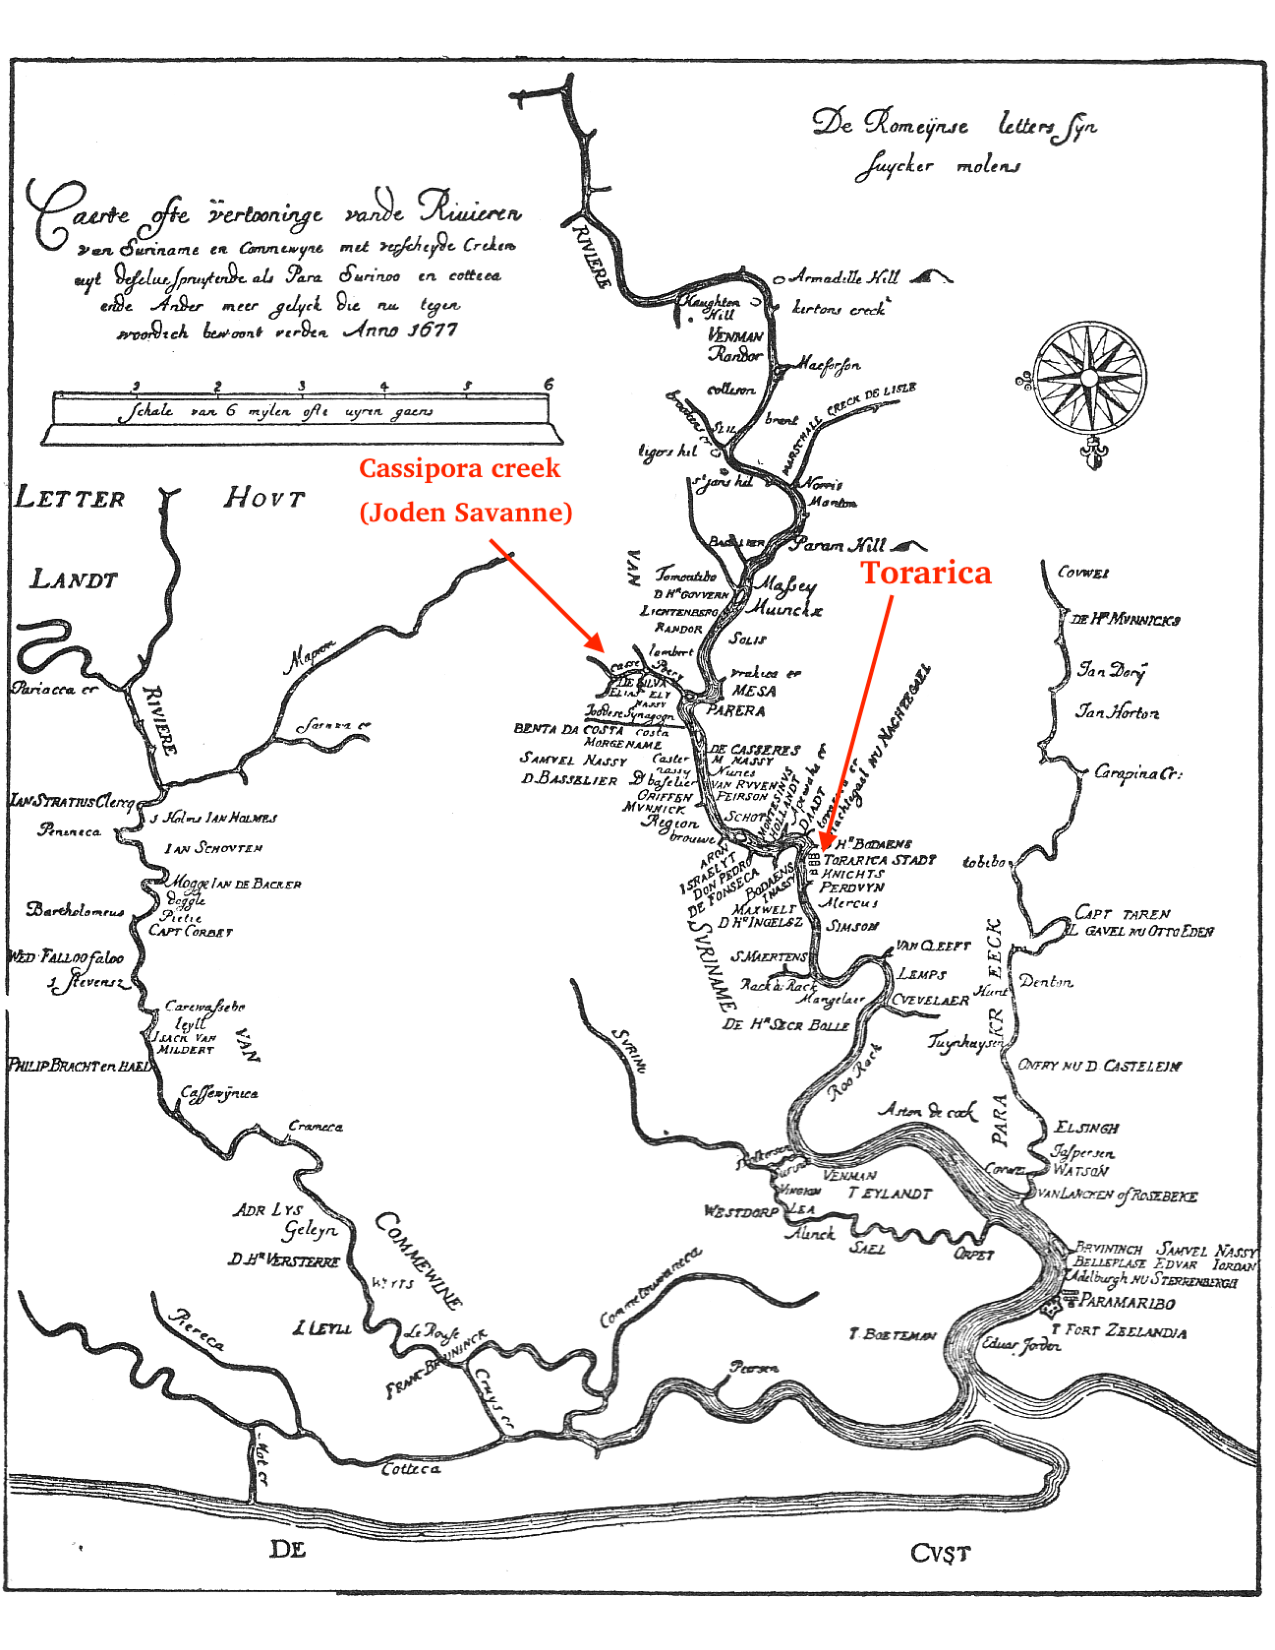
\includegraphics[width=\textwidth] {figures/1677kaartSurinameMogge.pdf}
% % % \captionsetup{name=Map}%
\caption {Location of plantations in late 17\textsuperscript{th} century Suriname. Source: \citet{Mogge77}} 
\label{Map1.1}
\end{figure}


In 1667, the \ili{Dutch}, led by Abraham Crijnssen, conquered \isi{Suriname} during the second Anglo-\ili{Dutch} War of 1665 to 1667. According to \citet{Hoefte98}, this war began because \isi{England} attempted to terminate the \ili{Dutch} dominance over world trade routes. On July 31, 1667, via the peace treaty of Breda, \isi{Suriname} was ceded to the \ili{Dutch} in exchange for New Amsterdam, which is present day New York \citep{Kaufman05}. Consequently, as allowed under the conventions of the Treaty of Breda \citep[617--618]{gbhol61}, most of the \ili{English} planters with enslaved Africans purchased before the cession to the \ili{Dutch}, alongside indentured servants and free \isi{Whites}, began leaving the mainland colony between 1668 and 1675 \citep{Arbell02, Faber98, Godfrey95}.

What was the linguistic situation while the \ili{English} were in control of the colony? How did this linguistic situation change with the arrival and subsequent settlement of the \ili{Portuguese}? What happened after the departure of the \ili{English} and arrival of the \ili{Dutch} and how did these social and linguistic changes contribute to the development of \ili{Sranan} Tongo?

\subsection {A change in the linguistic ecology of Suriname}\label{1.2.2}
The \ili{English} population in \isi{Suriname}, up until the commencement of their departure after 1667, consisted of planters, free \isi{Whites} and indentured servants who were coming from \isi{Barbados} \citep{Arbell02, Sainsbury80}. During the period of \ili{English} control, specifically between the period 1650 to 1664, i.e. the period prior to the introduction of the \ili{Portuguese} element into the colony, indentured servants from within the \ili{British} Isles constituted the bulk of the population in the \ili{English} colonies \citep{Kenny06, Powell05, Armitage05}. This is linguistically significant because these indentured servants ``formed the primary [\ili{English} \isi{Superstrate}] linguistic models'' \citep[117]{Arends02} for the enslaved Africans with whom they worked side by side on the plantations \citep{Galenson02}.

According to \citet{Rens53}, among the settlers going to \isi{Suriname} from \isi{Barbados}, some might have previously been residents of St. Kitts. This, according to \citet[117]{Arends02}, is very significant because St. Kitts was not only the first colony to be colonised by the \ili{English}, but it ``... may [also] have been the centre of diffusion of restructured \ili{English} throughout the \isi{Caribbean}, including \isi{Barbados}.'' It seems that it is for this reason that \citet{Arends02} holds the view that the \ili{English} roots of the Surinamese \ili{English}-\isi{lexicon} creoles should not be sought in \isi{Barbados} but in St. Kitts. I agree with \citet{Arends02} to an extent. However, given the migration patterns of indentured labourers from \isi{England} during the period in which \isi{Suriname} was settled, I would argue that \textsc{ssa}'s \ili{English} \isi{linguistic influence} is a combination of St. Kitts'  ``restructured \ili{English}'', alongside the \isi{linguistic influence}(s) from the indentured servants who arrived in \isi{Barbados} during the early 1650s onwards (see \chapref{ch:6}).

The linguistic ecology of \isi{Suriname} changed after 1664 with the arrival of the \ili{Portuguese} Jews, who established their plantations in close proximity to the \ili{English} ones. The subsequent linguistic situation had an effect on the \textsc{ssa}  creole \isi{languages} albeit in varying degrees (see \tabref{Table1.1}). According to \citet{Rens53}, the ``\il{Neger-English@``Neger-English''}Neger-English''  that was spoken in the colony by both the \ili{English} and enslaved Africans went through a process of fusion with the \ili{Portuguese} linguistic systems that the \ili{Portuguese} Jews and the enslaved took with them to \isi{Suriname}.

The linguistic ecology in \isi{Suriname} changed again in 1667 with the cession of the colony by the \ili{English} to the \ili{Dutch}. Barring runaway slaves, some of whom spoke ``\il{Neger-English@``Neger-English''}Neger-English'' and the few \ili{English} who had stayed, with most of the \ili{English} indentured servants, planters and ``\il{Neger-English@``Neger-English''}Neger-English''-speaking enslaved Africans leaving the colony, \isi{Suriname}'s linguistic ecology soon changed to one dominated by \ili{Portuguese} and \ili{Dutch}. Intriguingly, ``as far as the lexicons of the Surinamese \isi{Creoles} are concerned, it is an undisputed fact that \ili{English} ... [had] ... played a major role in their composition'' \citep[117]{Arends02}. Irrespective of the \ili{Portuguese} and \ili{Dutch} linguistic influences from 1667 onwards, the \ili{English} element was so deeply entrenched in the \textsc{ssa} creole \isi{languages} that even to date they can still be classified as \ili{English}-\isi{lexicon} creole \isi{languages}; this is illustrated in \tabref{Table1.1} below.

\begin{table}
\begin{tabular}{lrrrr} 
\lsptoprule
\textbf& \ili{English}  & \ili{Portuguese}  & \ili{Dutch} &  West African  \\
\midrule
\ili{Sranan} &  71.40\% & 3.70\% & 17.85\% & 1.59\%  \\
\ili{Aukan} &  76.47\% & 5.04\% & 15.97\% & 2.52\%  \\
\ili{Saramaccan} & 49.96\% & 34.88\% & 10.45\% & 4.74\%  \\  
\lspbottomrule 
\end{tabular}
\caption{Lexical sources of the 200-word basic vocabulary list for \textsc{ssa} }
\label{Table1.1}
\end{table}

 \tabref{Table1.1} does more than highlight the significance of the \ili{English} element based on a look at the 200-word basic vocabulary for the \textsc{ssa}  creole \isi{languages}; the table also highlights the fact that \ili{Dutch} had little \isi{linguistic influence} on the \textsc{ssa}  creole \isi{languages}. This lack of significant \isi{linguistic influence} from \ili{Dutch} is possibly attributable to the fact that the \ili{Dutch} were never able to implement, with any degree of success, the system of indentured servitude that the \ili{British} were able to establish \citep{Buddingh95}. Added to this is the fact that even though \ili{Dutch} became the official language of the colony and the ``language of literacy after emancipation,'' it was a language of high status that was seldom used to communicate with speakers of \ili{Sranan} (whether enslaved Africans or any of the \ili{English} who were in the country) during the 17\textsuperscript{th} and 18\textsuperscript{th} century \citep[279]{Healy93}.

The table also highlights another interesting fact, i.e. that the \ili{Portuguese} element, based on the 200-word basic vocabulary list, is far greater in \ili{Saramaccan} than the other two \textsc{ssa}  creoles. This has led some linguists, such as  \citet{Perl95}, to suggest that \ili{Saramaccan} should be classified as a \ili{Portuguese}-\isi{lexicon} creole language. Though this is not a position that I hold, this current work is not the medium through which to contest this claim. Let us therefore move to a brief discussion of the \isi{linguistic development} of \textsc{ssa}.

\subsection {Linguistic development of \textsc{ssa} }\label{1.2.3}
There are a number of elaborate explanations that various linguists have provided concerning the development of the \textsc{ssa}  creole \isi{languages}. This dissertation does not concern itself with which of these explanations is more valid and/or trustworthy. For this reason, the discussion hereafter is but a brief presentation of a few of them.

There are two major hypotheses that attempt to account for the development of the \textsc{ssa}  creole \isi{languages}; these are the Parallel Origin Hypothesis and the Serial Origin hypothesis \citep{Smith01}. According to the Parallel Origin Hypothesis, Proto-\ili{Sranan}, Proto-\ili{Saramaccan} and Proto-\ili{Aukan} developed independently, albeit from some type of \isi{Caribbean} Plantation Pidgin \ili{English}, hereafter \textsc{cppe}, which might have existed in the \ili{English} colonies during the first generation of slavery  \citep{Smith01, McWhorter98}. \textsc{cppe} possibly originated from an \ili{English} pidgin that might have been developed and spoken by castle slaves along the West African slave settlements \citep{McWhorter00b}.

According to \citet{McWhorter00b}, since all Atlantic \ili{English} \isi{Creoles} ``... must trace to a single ancestor, it is most likely that the pidgin was transported to ... St. Kitts and \isi{Barbados} [which were]... the first colonies settled [by the \ili{English}] and the source of settlers and slaves to subsequent [\ili{English}] colonies ...'' (111). This transported \ili{English} pidgin was possibly the same ``... embryonic Medium for Inter-ethnic Communication ...'' which according to \citet[347]{Baker98} existed in 1620s St. Kitts long before it became a first language and was spread to the other \ili{English} territories. In all likelihood \textsc{cppe} is the same as Baker's proposed mixed Afro-\ili{English} communication system \citep{Baker98}, which was spread to the other \ili{British} colonies including \isi{Suriname}; \textsc{cppe} might also be a further developed version of Baker’s Medium for Inter-ethnic Communication \citep{Baker98}, which developed due to the influence of the indentured servants coming into the colonies from the 1650s onwards (see \chapref{ch:6}).

The Serial Origin hypothesis also attributes the development of \textsc{ssa}  to \textsc{cppe}. However, Proto-\ili{Sranan} is considered to be the first to develop from \textsc{cppe}, within \isi{Suriname}, followed by \ili{Aukan} and \ili{Saramaccan} as offshoots from \ili{Sranan} \citep{Smith01, McWhorter98}. Shortly after \textsc{cppe} was transported to \isi{Suriname}, \ili{Sranan} developed, before \ili{Saramaccan} and \ili{Aukan}, due to the continual contact between enslaved Africans, ``... indentured servants and poor whites, who acted as bookkeepers and overseers on the plantations ...'' \citep[xii]{Cassidy67}. This \ili{English}, indentured servant-based, \isi{linguistic influence} would certainly have lasted only until just after 1668, with the departure of the \ili{English}.

\citet{Smith09, Smith06, Smith02} argued that \ili{Sranan} developed in the first half of the 1660s. In fact, \citet[316]{Smith09} ``... [dated] the creolization of \ili{Sranan} at 1660--1665.'' This means that by the time of the arrival of the \ili{Portuguese} Jews in 1664, \ili{Sranan} or some semblance of it was already created. Smith's claim is supported by \citet[28]{Rens53} who claimed that prior to the arrival of the \ili{Portuguese} Jews in \isi{Suriname}, ``\il{Neger-English@``Neger-English''}Neger-English'' had long been established among the enslaved Africans and white inhabitants of the country.

\ili{Sranan}, by around 1680--1690, was partly relexified by \ili{Portuguese}. This is attributed to the influence of \ili{Portuguese} Jewish immigrants who were granted asylum in 1664  \citep{McWhorter11, Smith06, Holm89}. According to  \citet[156]{Smith08b}, these \ili{Portuguese} Jews had brought ``\ili{Portuguese} speaking slaves with them to \isi{Suriname}'' when they first entered the then \ili{English} colony. At some point there was a fusion of what \citet{Rens53} called Neger-\ili{Portuguese}, spoken by the \ili{Portuguese} enslaved Africans, and the \il{Neger-English@``Neger-English''}Neger-English spoken by the \ili{English} enslaved Africans and some of the indentured servants. This possibly took place during and after 1667, when the \ili{Portuguese} Jews purchased \ili{Sranan} (\il{Neger-English@``Neger-English''}Neger-English) speaking enslaved Africans from the \ili{English} who were preparing to migrate from \isi{Suriname} due to its having been ceded to the \ili{Dutch} \citep{Ehrlich09, Mufwene01, Friedman99, McWhorter98, Wurm96, Rens53}. This fusion of the two \isi{languages} saw the birth of a kind of Dju-Tongo (Jew language), a mixed \ili{Portuguese}/\ili{English} creole, in the middle of the \isi{Suriname} River plantations \citep{Arends95}.

By the 1690s, the first group of enslaved Africans ran away from the \ili{Portuguese} Jewish plantations to form the first \ili{Saramaccan} group in the interior of the country \citep{Huber99}. The high percentage of \ili{Portuguese} lexical items in \ili{Saramaccan} (see \tabref{Table1.1} on Page~\pageref{Table1.1}) is attributed to this Dju-Tongo, which according to \citet{Arends95} ``... [involved] the same mix of \ili{English}, \ili{Portuguese} and African elements as \ili{Saramaccan}...'' (169).

\ili{Aukan} (commonly referred to as \ili{Ndjuka} or \ili{Djuka}) ``... is lexically more similar to \ili{Sranan}''  \citep[Introduction]{Huttar94}. \citet{Huttar94} claimed that this creole language variety appeared in the first half of the 18\textsuperscript{th} century, when ``large numbers of slaves escaped from plantations chiefly along the Cottica and Commewijne rivers where a \isi{contact language} drawing much of its \isi{lexicon} from \ili{English} was in use'' \citep[Introduction]{Huttar94}. This \isi{contact language} is what \citet{McWhorter98}  considered to be \ili{Sranan}.

Since most of the \ili{English} would have already migrated from \isi{Suriname} by 1680, resulting in \ili{Sranan}'s linguistic ecology being one that was dominated by \ili{Portuguese} and \ili{Dutch}, how do we account for \ili{Aukan} being similar to \ili{Sranan}? How can we account for \ili{Sranan} still being spoken as the \isi{lingua} franca today, as opposed to \ili{Saramaccan} or some \ili{Dutch}-based creole that is a fusion of \ili{Dutch} and Neger \ili{English} (\ili{Sranan})? According to \citet{Holm94} the \ili{Dutch} in \isi{Suriname} treated \ili{Sranan} as a language in its own right, though not one of prestige. Consequently, they learned it as a second language to communicate with their enslaved Africans, some of whom were acquired from the migrating \ili{English} after \isi{Suriname}?s cession to the \ili{Dutch} (see \chapref{ch:6}).

This work does not attempt to settle which of the two hypotheses, i.e. the Parallel Origin Hypothesis or the Serial Origin Hypothesis, is more trustworthy. What is important is the fact that \textsc{ssa}, specifically \ili{Sranan}, contains what might be considered ``fossilized'' linguistic remnants of an early \ili{English} colonial period. Therefore, it is being proposed here, that these linguistic ``fossils'' can be used to trace the dialect origin(s), in \isi{England}, of the early \ili{English} influence.
%section 1.2 ends %%%%%%%%%%%%%%%%%%%%%%%%%%%%%%%%%%%%%%%%%%%%%%%%%%%%%%%%%%%%%%%%%%%%%

%section 1.3 starts %%%%%%%%%%%%%%%%%%%%%%%%%%%%%%%%%%%%%%%%%%%%%%%%%%%%%%%%%%%%%%%%%%%%%
\section{The problem} \label{1.3}

Though linguists, such as \citet{Smith08, Smith87} and \citet{Mufwene08, Mufwene01}, present 17\textsuperscript{th} century \isi{dialects} of \ili{English} as the lexical input for \ili{English} creoles, Smith was more specific regarding the nature of this input. He posited dialect levelling involving an approximation of an emerging 17\textsuperscript{th} century ``... London \ili{English}, primarily Standard Early Modern \ili{English} ...'' \citep[118]{Smith08}. He held this view because he believed that ``... the \ili{English} that developed in the general London area [was] ancestral to all forms of \ili{English} developed external to the \ili{British} Isles ...'' \citep[118]{Smith08}. He supported this claim by tracing systematic sound changes based on south-east \isi{England} \ili{English} input and their realisations in \isi{Suriname}. \citet{Smith08, Smith87} did not, however, present evidence to repudiate the possibility of a \isi{pan-dialectal account} of origin, i.e. the possibility that the origin of this influence was coming from \isi{dialects} from all over \isi{England}. This latter view is endorsed by \citet{Mufwene08, Mufwene01}.

\citet{Mufwene08, Mufwene01} believed that ``... the target for those who made the creoles, consisted of several non-standard [dialect] varieties [of the European lexifiers that were] competing with each other ...'' \citep[21]{Mufwene08}. Like \citet{Smith08, Smith87}, \citet{Mufwene08, Mufwene01} failed to provide any assessment of the possibility of an alternative account to his pan-dialectal one; i.e. he did not address the possibility of a mono-dialectal source of origin, such as that proposed by \citet{Smith08, Smith87}.
%section 1.3 ends %%%%%%%%%%%%%%%%%%%%%%%%%%%%%%%%%%%%%%%%%%%%%%%%%%%%%%%%%%%%%%%%%%%%%

%section 1.4 starts %%%%%%%%%%%%%%%%%%%%%%%%%%%%%%%%%%%%%%%%%%%%%%%%%%%%%%%%%%%%%%%%%%%%%
\section {Significance of research}\label{1.4}
This research attempts to settle the pan-dialectal and the mono-dialectal contention surrounding the nature of the historical \isi{lexico-phonetic input} in \ili{English} creoles, specifically \ili{Sranan}. To this end, it puts forward a methodological apparatus that one can use to undertake such reconstructive work and achieve replicable results. This methodological tool involves a combination of \isi{statistics} (\chapref{ch:4}), \ili{English} \isi{dialect geography} (\chapref{ch:5}) and 17\textsuperscript{th} century history of \isi{England} (\chapref{ch:6}).
%section 1.4 ends %%%%%%%%%%%%%%%%%%%%%%%%%%%%%%%%%%%%%%%%%%%%%%%%%%%%%%%%%%%%%%%%%%%%%

%section 1.5 starts %%%%%%%%%%%%%%%%%%%%%%%%%%%%%%%%%%%%%%%%%%%%%%%%%%%%%%%%%%%%%%%%%%%%%
\section{Outline of chapters}\label{1.5}
\chapref{ch:2}, \emph{Brief overview: Views on \isi{superstrate} influence}, begins with a brief discussion of the theories of \isi{creole genesis} that exist to date. The discussion then looks specifically at two superstratist approaches of origin which offer opposing ideas about the nature of the \isi{superstrate} input; it then focuses specifically on the \isi{superstrate influence} in \ili{Sranan}. The discussion concludes with an explanation and rationale for the direction that this research takes in attempting to establish what \ili{Sranan}'s \isi{linguistic influence} from \isi{England} looks like and how best to account for it.

\chapref{ch:3}, \emph{About the data and research design}, is divided into two major sections. The first section, \emph{Data Sources}, is a discussion and presentation of the \ili{Sranan}, the \ili{English} of \isi{England}, 17\textsuperscript{th} century history of \isi{England} data sources and the \isi{linguistic features} assessed in this research. The second section, \emph{Research Design}, is a detailed discussion and presentation of:

\begin{enumerate}
\renewcommand{\labelenumi}{\alph{enumi}.} 
\item the approach taken in gathering, organising and using the \ili{English} \isi{regional dialect} data and the \ili{Sranan} data; and
\item the processes that took place at each stage of the proposed tripartite methodological model used to undertake this research.
\end{enumerate}

\chapref{ch:4}, \emph{Testing \isi{probability} of origin}, is a presentation of the statistical component of the methodological apparatus at work, using 45 putative lexico-pho\-net\-ic \ili{English} etyma, hereafter the \textsc{sed45}, which have been selected for this research (see \chapref{ch:3}). The chapter discusses the \isi{probability} of finding a single dialect locality of origin, which exhibits a high degree of correspondence between the 45 \isi{putative input etyma} and their \ili{Sranan} reflexes, hereafter referred to as the Sranan45. It then looks at the significance of actually finding a single such locality of origin from within \isi{England} and subsequently presents the actual results of the statistical analysis.

\chapref{ch:5}, \emph{A \isi{dialect geography} approach}, is a presentation and discussion of potential locations of origin in \isi{England} of the \ili{English} reflexes for the Sranan45. In this chapter, the results of the statistical analysis presented in \chapref{ch:4} are temporarily disregarded and the data are analysed anew within a \isi{dialect geography} framework. This involves plotting on a map of \isi{England} the \isi{geo-linguistic distribution} of the \textsc{sed45} etyma. The chapter concludes with a discussion of the degree of corroboration between the results of the \isi{geo-linguistic mapping} and the results of the statistical analysis of the  \textsc{sed45}.

\chapref{ch:6}, \emph{The historical complement}, is a discussion of the 17\textsuperscript{th} century migration patterns of people from \isi{England} going to \ili{British} colonies in the Americas. The focus of the discussion is on the patterns of migration from the locations identified via the statistical analysis and the \isi{geo-linguistic mapping} as the potential sources for the Sranan45. The discussion is concerned with answering three main questions that are posed at the end of \chapref{ch:5}. These are as follows:

\begin{enumerate}
\item Can we establish a chain of migration from \isi{England} to \isi{Suriname}, between the periods 1650--1667?
\item Can we establish a chain of migration from \isi{England}, within the same time span mentioned in (1), to the \ili{English} colonies in the \isi{Caribbean} and subsequently \isi{Suriname}?
\item Can we, if the answer(s) to (1) and/or (2) is/are in the affirmative, then determine what percentage of the total number of migrants to the \isi{Caribbean}, including \isi{Suriname}, is from the localities pinpointed in Chapters~\ref{ch:4} and~\ref{ch:5}?
\end{enumerate}

\chapref{ch:7}, \emph{A Tale of Two Dialect Inputs}, is a discussion of the composite findings from the three components of the analytical tool (see Chapters~\ref{ch:4}--\ref{ch:6}). This final chapter also looks at the significance of these combined findings as they relate to \ili{Sranan}, Linguistic reconstruction, Dialect \isi{geography}, \ili{Creole} and Historical Linguistics and \ili{English}-\isi{lexicon} creole \isi{languages} in general.
%section 1.5 ends %%%%%%%%%%%%%%%%%%%%%%%%%%%%%%%%%%%%%%%%%%%%%%%%%%%%%%%%%%%%%%%%%%%%%
